\section{Representación Gráfica}\index{Gráficos}
La posibilidades gráficas constituyen, junto a la facilidad para manejar matrices, uno de los aspectos más atractivos de Matlab como herramienta de cálculo científico. Matlab permite realizar gráficos en dos y tres dimensiones de muy diversos tipos. 

\subsection{El comando plot y las figuras en Matlab.}\index{Gráficos!Plot}
\paragraph{plot.} El comando de dibujo más sencillo de Matlab es el comando \texttt{plot}. La filosofía de dibujo es muy sencilla se pasan como variables de entrada dos vectores, el primero de ellos con las coordenadas \texttt{x} y el segundo con las correspondientes coordenadas \texttt{y} de los puntos que se desea dibujar. Si no se indica nada, Matlab unirá los puntos mediante líneas rectas. Supongamos que deseamos representar gráficamente los puntos $(x,y)$ de la siguiente tabla de datos,

\begin{table}[h]
\caption{Datos de prueba}
\centering
\begin{tabular}{|c|c|}
x&y\\ 
\hline
0&0\\
2&3\\
-1&2\\
-2&-4\\ 
\end{tabular}
\label{tpuntos}
\end{table} 

Para ello, lo primero que hacemos es construir dos vectores; uno con las coordenadas x de los puntos,
\begin{verbatim}
>> x=[0 2 -1 -2]
x =

     0     2    -1    -2

\end{verbatim}
y el otro con las coordenadas y de los puntos,
\begin{verbatim}
>> y=[0 3 2 -4]
y =

     0     3     2    -4
\end{verbatim}
 
Por último empleamos el comando \texttt{plot}, dando como variables de entrada los dos vectores construidos,
 
\begin{verbatim}
>> plot(x,y)
\end{verbatim}

Matlab responde al comando abriendo una ventana gráfica, como la que muestra la figura \ref{fig:ventana}, con la figura correspondiente a los puntos de la tabla, unidos mediante líneas rectas.

\begin{figure}[h]
\centering
\includegraphics[width=12cm]{figura.png}
\caption{Ventana gráfica de Matlab. representación de los punto de la tabla \ref{tpuntos}}
\label{fig:ventana}
\end{figure}

La ventana gráfica de Matlab, tiene en su parte superior una barra de herramientas y un menú desplegable con funciones específicas para la manipulación de los gráficos. Se aconseja leer la ayuda de Matlab sobre el uso de dichas herramientas.

Una de las opciones del menú desplegable, permite guardar la figura generada como un archivo gráfico. Además, es posible mediante otra de las opciones del menú copiar la figura y pegarla posteriormente en un editor de texto\footnote{Al menos es posible hacerlo así si se trabaja en el sistema operativo Windows de Microsoft.}. Si copiamos la figura \ref{fig:ventana} y la pegamos directamente en el texto obtendríamos un gráfico como el de la figura, \ref{fig:plot}. A partir de ahora importaremos de esta manera todas las figuras que construyamos con Matlab.

\begin{figure}[h]
\centering
\includegraphics[width=12cm]{plot.eps}
\caption{gráfico de los puntos de la tabla \ref{tpuntos} obtenida con el comando \texttt{plot}}
\label{fig:plot}
\end{figure}
El comando plot admite un tercer parámetro de entrada. Se trata de símbolos, escritos entre comillas simples, que permiten definir: 
\begin{itemize}
\item El tipo de línea que se empleará en el gráfico. por ejemplo \texttt{plot(x,y,'-.`')} une los puntos mediante una línea de puntos y guiones.
\item El símbolo que se empleará para representar los puntos. Por ejemplo, \texttt{plot(x,y,'o')} dibuja un círculo en la posición de cada punto y no los une entre sí mediante líneas rectas.
\item El color que se empleará para dibujar. Por ejemplo, \texttt{plot(x,y,'r')}. Dibuja la gráfica en color rojo.
\end{itemize}

Si no se define este tercer parámetro, \texttt{plot} dibujará los gráficos, por defecto, en color azul, uniendo los puntos con líneas continuas y no usará ningún símbolo para dibujar los puntos individuales.
 
La tabla \ref{tcolor} muestra los símbolos disponibles para dibujar con el comando \texttt{plot}.

\begin{table}[h]
\caption{tipos de línea y color del comando \texttt{plot}}
\centering
\begin{tabular}{rc|rc|rc}
Tipo de línea&Símbolo&Tipo de punto& Símbolo &Color&Símbolo\\ 
\hline
continua&-&punto&.&azul&b\\
puntos&:&círculo&o&verde&g\\
puntos y guiones&-.&equis&x&rojo&r\\
guiones&--&más&+&cyan&c\\
&&asterisco&*&amarillo&y\\
&&diamante&d&negro&k\\
&&triangulo vértice abajo&v&blanco&w\\
&&triangulo vértice arriba&\^{}&&\\
&&triangulo vértice izquierda&\textless&&\\
&&triangulo vértice derecha&\textgreater&&\\
&&triangulo vértice arriba&\^{}&&\\
&&cuadrado&s&&\\
&&pentágono&p&&\\
&&hexágono&h&\\
\hline
\end{tabular}
\label{tcolor}
\end{table} 

Se puede combinar un símbolo de cada tipo en un mismo \texttt{plot}. Así por ejemplo si queremos representar los datos de la tabla \ref{tpuntos} unidos mediante una línea de puntos,
\begin{verbatim}
plot(x,y,':')
\end{verbatim} 

Si queremos que pinte solo los puntos sin unirlos con líneas y en color rojo,
\begin{verbatim}
plot(x,y,'.r')
\end{verbatim}

Si queremos que pinte los puntos representados por triángulos con el vértice hacia arriba, unidos mediante una línea continua y en color negro,

\begin{verbatim}
plot(x,y,'-^k')
\end{verbatim}

La figura \ref{fig:tplot} muestra los resultados de las combinaciones de símbolos que acabamos de describir.

\begin{figure}[h]
\centering
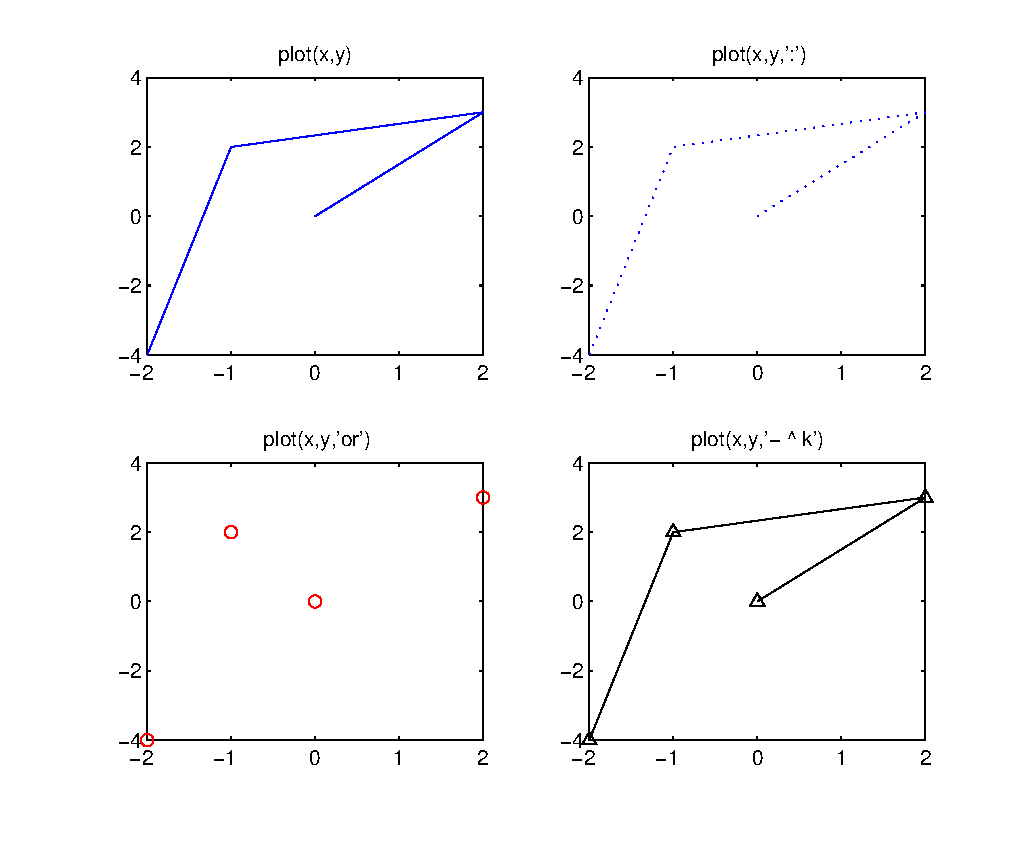
\includegraphics[width=12cm]{tiposplot.eps}
\caption{Datos de la tabla \ref{tpuntos} representados mediante distintos tipos de líneas y colores}
\label{fig:tplot}
\end{figure}

\paragraph{Figuras.} Cada vez que escribimos en la ventana de comandos de Matlab, un comando gráfico como por ejemplo \texttt{plot} Matlab comprueba si existe alguna figura (ventana de gráficos) abierta. Pueden darse entonces tres situaciones distintas. 

\begin{enumerate}
\item No hay ninguna figura abierta. Matlab crea entonces una figura nueva y representa en ella el gráfico pedido.
\item Hay una figura abierta. Matlab empleará dicha figura para representa el gráfico pedido. Por defecto, Matlab borrará cualquier gráfico anterior que contuviese la figura.
\item Existe más de una figura abierta. Matlab empleará para dibujar la llamada figura activa, que corresponde con la figura que se haya utilizado o que se haya seleccionado por última vez con el ratón.
\end{enumerate}

Es posible crear varias figuras distintas empleando directamente el comando \texttt{figure}. Cada vez que lo introduzcamos en la ventana de comandos, Matlab creará una figura nueva asignándole un número (figura 1, 2 ,3 etc.). Si empleamos el comando \texttt{figure}, seguido de un número entre paréntesis, \texttt{figure(25)}, Matlab creará una nueva figura asignándole dicho número y si ya existe la figura la convertirá en la figura activa.
El siguiente script muestra un ejemplo del uso de \texttt{figure} y \texttt{plot} combinados.

% \begin{lstlisting}
% % este script  (figuras.m)muestra el uso de los comandos figure y plot 
% % para pintar varias funciones se aconseja copiarlo y probarlo en 
% % Matlab para entender mejor cómo funciona.

% % vamos a pintar un trozo de la función e^x, en concreto para el 
% % intervalo x=[0,1]

% % Construimos un vector de 100 puntos equiespaciados en el intervalo [0,1]

% x=linspace(0,1,100);

% % calculamos el valor de la funcion e^x para los puntos construidos,

% y1=exp(x);

% % pintamos los puntos y frente a x,

% plot(x,y1) % plot ha construido una figura en Matlab, la figura 1.

% % Construimos una segunda figura en Matlab
% figure % se ha construido la figura 2

% % construimos una tercera figura 
% figure % se ha construido la figura 3


% % calculamos los valores que tomará la función sin(2*pi*x) para los 
% % puntos x del intervalo [0,1] que ya tenemos
% y2=sin(2*pi*x);

% % hacemos activa la figura 2
% figure(2)
% % pintamos en esta figura los puntos de la función sin...

% plot(x,y2)

% % volvemos a hacer activa la figura 1
% figure(1)
% % pintamos ahora los puntos de la de la función y=e^x, pero invertidos 
% % x frente a y, La grafica anterior se borra y es sustituida por la nueva,
% plot(y1,x)

% % creamos una nueva figura asignándole un numero al crearla,
% figure(13)

% % volvemos activar la figura 3
% figure(3)

% % volvemos a pintar, ahora en la figura 3, la función y=e^x,
% plot(x,y1)

% % volvemos a activar la figura 13 y pintamos en ella de nuevo la 
% % funcion sin..

% figure(13)
% plot(x,y2)
% \end{lstlisting}

Como se ha señalado antes, cualquier comando gráfico que se ejecute borra por defecto el contenido anterior de la figura activa. Es posible cambiar este comportamiento, empleando para ello el comando \texttt{hold}. Si en la ventana de comandos escribimos \texttt{hold on}, a partir de ese momento la ventana activa mantendrá cualquier gráfico que contenga y añadirá a este los nuevos gráficos que se creen. Este comportamiento se mantiene hasta que vuelva a escribirse en la ventana de comandos la sentencia \texttt{hold off}. El siguiente script muestra un ejemplo del uso de este comando y La figura \ref{fig:sico} el gráfico resultante.

% \begin{lstlisting}
% % ejemplo de uso de hold on para representar dos funciones en el mismo
% % gráfico

% % vamos a representar las funciones seno y coseno en el intervalo [-pi, pi]

% % creamos un vector de 100 puntos en el intervalo,
% x=[-pi:2*pi/99:pi];

% % calculamos el valor de la función seno sobre los puntos x
% seno=sin(x);

% % calculamos el valor de la función coseno sobre los puntos x
% coseno=cos(x);

% % pintamos la funcion seno, con linea continua azul
% plot(x,seno)

% % le pedimos que mantenga el gráfico creado
% hold on

% % pintamos encima la función coseno en linea continua roja

% plot(x,coseno,'r')

% \end{lstlisting}


\begin{figure}[h]
\centering
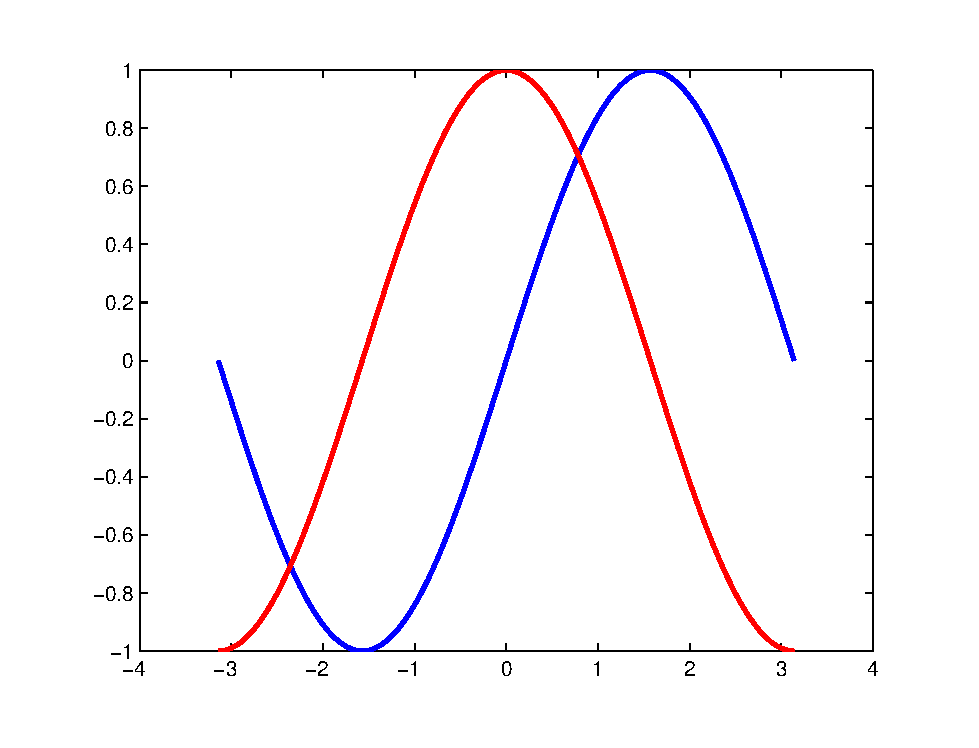
\includegraphics[width=12cm]{sico.eps}
\caption{gráficas de las funciones seno y coseno en el intervalo $(-\pi, \pi)$. Representadas en la misma figura, usando el comando \texttt{hold on}.}
\label{fig:sico}
\end{figure}

Es posible también incluir varios gráficos separados en la misma figura. 
Para ello se emplea el comando \texttt{subplot(i,j,k)}. Este comando divide la figura en un total de $i\times j$ gráficos y activa el situado en la posición $k$, las posiciones se cuentan fila a fila de arriba a abajo. El siguiente script muestra el uso del comando \texttt{subplot} La figura \ref{fig:subplot} muestra el resultado obtenido.
\begin{figure}[h]
\centering
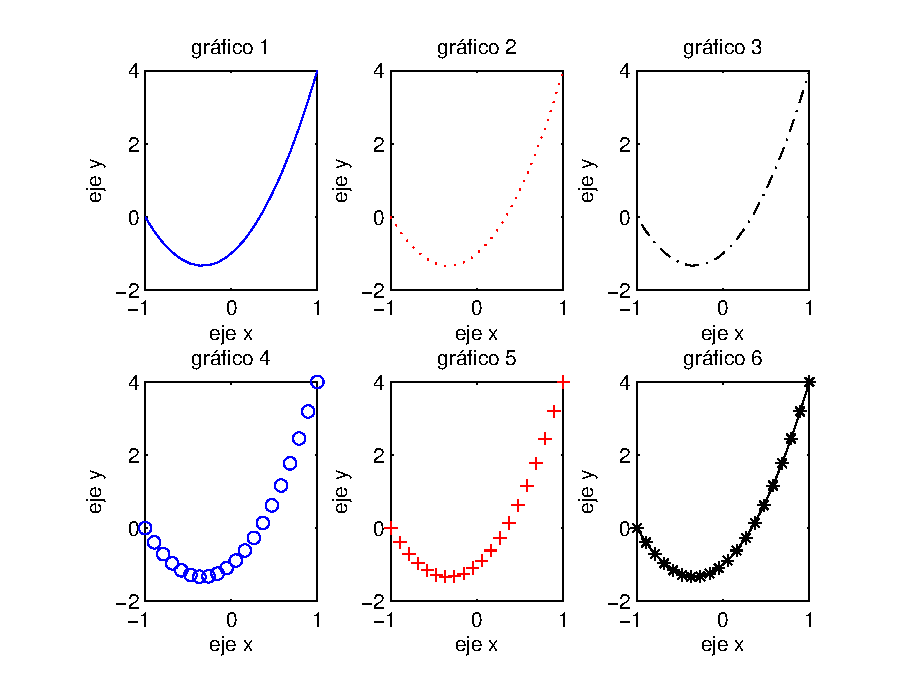
\includegraphics[width=12cm]{subplot.eps}
\caption{Ejemplo de empleo del comando subplot}
\label{fig:subplot}
\end{figure}


% \begin{lstlisting}
% % Este script muestra el uso del comando subplot

% % vamos a crear una figura con 2X3=6 gráficas, se disponen en la figura 
% % como si fueran los elementos de una matriz...
% % usamos el comando subplot de modo que cree el primer eje de los 6
% subplot(2,3,1)

% % definimos un vector x de puntos equiespacios en el intervalo (-1,1)
% x=linspace(-1,1,20);

% % calculamos los valores de polinomio 3x^2+2^x-1
% y=3*x.^2+2*x-1;

% % dibujamos la función en los ejes
% plot(x,y)

% % Añadimos rótulos a los ejes
% xlabel('eje x')
% ylabel('eje y')
% % Añadimos un titulo al grafico
% title('gráfico 1')

% % Generamos los siguientes ejes (a la derecha del anterior)
% subplot(2,3,2)
% % dibujamos la misma función pero ahora en linea discontinua roja
% plot(x,y,':r')

% % Añadimos rótulos a los ejes
% xlabel('eje x')
% ylabel('eje y')
% % Añadimos un titulo al grafico
% title('gráfico 2')

% % Generamos los siguientes ejes (a la derecha del anterior)
% subplot(2,3,3)
% % dibujamos la misma función pero ahora en linea de punto y raya negra
% plot(x,y,'-.k')

% % Añadimos rótulos a los ejes
% xlabel('eje x')
% ylabel('eje y')
% % Añadimos un titulo al grafico
% title('gráfico 3')

% % Generamos los siguientes ejes (debajo de los primeros)
% subplot(2,3,4)
% % dibujamos la misma función pero ahora solo con circulos azules
% plot(x,y,'o')

% % Añadimos rótulos a los ejes
% xlabel('eje x')
% ylabel('eje y')
% % Añadimos un titulo al grafico
% title('gráfico 4')

% % Generamos los siguientes ejes (a la derecha del anterior)
% subplot(2,3,5)
% % dibujamos la misma función pero ahora solo con cruce rojas
% plot(x,y,'+r')

% % Añadimos rótulos a los ejes
% xlabel('eje x')
% ylabel('eje y')
% % Añadimos un titulo al grafico
% title('gráfico 5')

% % Generamos los últimos ejes (a la derecha del anterior)
% subplot(2,3,6)
% % dibujamos la misma función pero ahora en linea continua y asteriscos
% % negros
% plot(x,y,'-*k')

% % Añadimos rótulos a los ejes
% xlabel('eje x')
% ylabel('eje y')
% % Añadimos un titulo al grafico
% title('gráfico 6')
% \end{lstlisting}


En el ejemplo, se ha hecho usos de algunos comandos para gráficos que permiten introducir títulos. Estos son: 

\texttt{title}, introduce un titulo a un gráfico, por ejemplo,
\begin{verbatim}
title('gráfico de temperaturas')
\end{verbatim}

\texttt{xlabel}, añade un rótulo al eje x, por ejemplo,

\begin{verbatim}
xlabel('tiempo en segundos')
\end{verbatim}

\texttt{ylabel} añade un rótulo al eje y , por ejemplo,
\begin{verbatim}
ylabel('distancia en metros')
\end{verbatim}

\subsection{Gráficos en 2D} \index{Gráficos! Comandos gráficos en 2D}
Hasta ahora, hemos visto tan solo el comando \texttt{plot}, que nos ha servido para introducir las capacidades gráficas en Matlab. Como hemos visto, plot permite representar gráficamente colecciones de datos en dos dimensiones. Hay otros muchos comandos que permiten obtener representaciones \emph{especializadas} de datos en dos dimensiones. A continuación veremos algunos de los más destacables.
\begin{figure}[h]
\centering
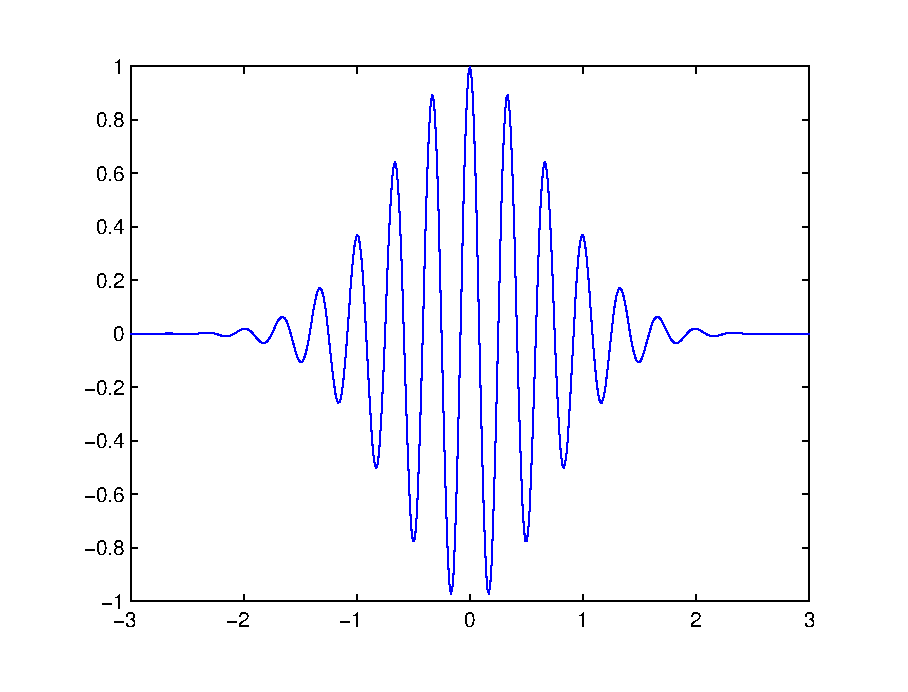
\includegraphics[width=12cm]{wave.eps}
\caption{Ejemplo de empleo del comando \texttt{fplot}}
\label{fig:wave}
\end{figure} 

\paragraph{fplot.} Permite dibujar directamente una función en un intervalo de valores. El nombre de la función hay que introducirlo entre comillas simples y el intervalo como un vector de dos componentes. Por ejemplo,

\begin{verbatim}
>> fplot('exp(-x.^2).*cos(6*pi*x)',[-3 3])
\end{verbatim}

dibuja la función,
\begin{equation*}
f(x)=e^{-x^2}\cos(6\pi x)
\end{equation*}

en el intervalo $[-3,3]$ (figura \ref{fig:wave}).

 
\paragraph{semilogx.} El comando \texttt{semilog} representa el eje de las x en escala logarítmica, Es decir, en lugar de representar frente a la variable $x$, se representa frente a $\log_{10}(x)$. Si dibujamos empleando este tipo de gráfico la función $y=\log_{10}(x)$ deberíamos obtener una línear recta de pendiente unidad. La figura \ref{fig:slx} muestra el resultado, empleando para las \emph{equis} el intervalo $(0,1)$.
\begin{verbatim}
>> x=linspace(0,1,100);
>> y=log10(x);
>> semilogx(x,y)
>> grid on
\end{verbatim}

\begin{figure}[h]
\centering
\includegraphics[width=10cm]{slx.eps}
\caption{Representación de la función $y=\log_{10}(x)$ empleando el comando \texttt{semilogx}}
\label{fig:slx}
\end{figure} 

Un par de observaciones sobre este ejemplo: En primer lugar las divisiones del eje x aparecen marcadas como potencias de 10. Como estamos representando empleando el logaritmo decimal de la variable x, las divisiones se corresponden con el exponente de la potencia de 10 de cada división, $\log_{10}(10^n)=n$.

En segundo lugar hemos empleado un nuevo comando gráfico; se trata del comando \texttt{grid}. Este comando añade una retícula al gráfico de modo que sea más fácil ver los valores que toman las variables en cada punto de la gráfica. \texttt{grid on},añade la retícula y \texttt{grid off} la retira.

\paragraph{semilogy.} Análoga al anterior, simplemente que ahora es el eje y el que se representa en escala logarítmica. En este caso será si representamos la función $y=10^x$ cuando obtengamos una línea recta,

\begin{verbatim}
>> x=linspace(0,1,100);
>> y=10.^x;
>> semilogy(x,y)
>> grid on
\end{verbatim}

\begin{figure}[h]
\centering
\includegraphics[width=10cm]{sly.eps}
\caption{Representación de la función $y=10^x$ empleando el comando \texttt{semilogy}}
\label{fig:sly}
\end{figure}

\paragraph{loglog.} Análoga a las anteriores, \texttt{loglog(x,y)} representa \texttt{y} frente a \texttt{x} empleando en ambos ejes una escala logarítmica.


\paragraph{polar.} Representa funciones en coordenadas polares \texttt{polar(theta,r}. La primera variable es un ángulo en radianes y la segunda el correspondiente radio. La figura \ref{fig:esp} muestra la espiral,
\begin{equation*}
r=2\cdot\sqrt{\theta}
\end{equation*}

Para el intervalo angular $[0,8\pi]$.
 
\begin{verbatim}
>> theta=linspace(0,8*pi,100);
>> r=2*theta;
>> polar(theta,r)
>> r=sqrt(theta);
>> polar(theta,r)
\end{verbatim}

\begin{figure}[h]
\centering
\includegraphics[width=10cm]{esp.eps}
\caption{Representación de la función $r=\sqrt{\theta}$ empleando el comando \texttt{polar}}
\label{fig:esp}
\end{figure}

\paragraph{stem, bar, stairs.} En los tres casos, se obtienen representaciones \emph{discretas} de un conjunto de datos. \texttt{stem} representa los datos mediante líneas verticales que parten del eje  x y llegan hasta el valor correspondiente de y. Las líneas van rematadas por un círculo. \texttt{bar} Emplea barras solidas verticales  y \texttt{stairs} realiza una representación en escalera. La figura \ref{fig:sbs} muestra el resultado de dibujar, empleando estos tres tipos de gráficos, los datos correspondientes al número de coches por cada 1000 habitantes en 2007 para cincuenta países distintos (los datos se guardaban en una matriz llamada auto\_50\_2007),

\begin{verbatim}
>> subplot(1,3,1)
>> stem(auto_50_2007)
>> subplot(1,3,2)
>> bar(auto_50_2007)
>> subplot(1,3,3)
>> stairs(auto_50_2007)
\end{verbatim}

\begin{figure}[h]
\centering
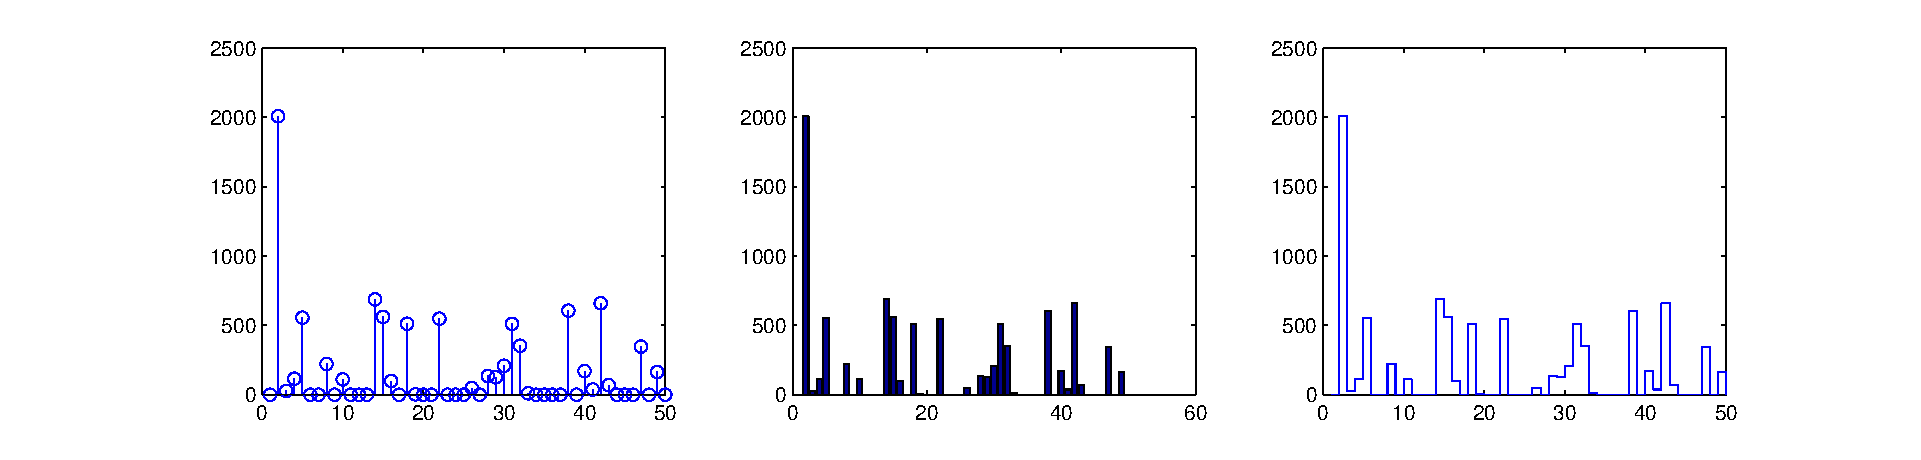
\includegraphics[width=15cm]{sbs.eps}
\caption{Comparción entre los comandos \texttt{stem}, \texttt{bar} y \texttt{stairs} representando la misma colección de datos.}
\label{fig:sbs}
\end{figure}

\paragraph{hist.} Este comando permite dibujar el histograma de una colección de datos. El histograma es una forma de representar cuantas veces se repite un datos, o más exactamente cuantos datos de la colección caen dentro de un intervalo dado. La función \texttt{hist(x,n)} admite dos parámetros de entrada, un vector de datos \texttt{x} y un valor entero \texttt{n} que representa el número de intervalos en que se dividirá el rango de valores de \texttt{x}, para obtener el histograma. Si no se introduce esta segunda variable, Matlab por defecto divide el rango de los datos en 10 intervalos. Veamos un ejemplo de uso de hist, empleando los datos del ejemplo anterior relativos a número de coches por cada mil habitantes. Representaremos el histograma para un total de 213 países. Para tener una idea, del rango de los dato, calculamos el valor mínimo y máximo de los datos disponibles,
\begin{verbatim}
>> minimo=min(auto2007)
minimo =

     0

>> maximo=max(auto2007)

maximo =

   874
\end{verbatim}

El rango va de $0$ a $879$ automóviles por cada mil habitantes. La figura \ref{fig:hist} muestra los histogramas obtenidos sin indicar el número de intervalos, ---por lo que se tomarán 10---, tomando 5 intervalos y tomando 20.

\begin{verbatim}
>> subplot(1,3,1)
>> hist(auto2007)
>> subplot(1,3,2)
>> hist(auto2007,5)
>> subplot(1,3,3)
>> hist(auto2007,20)
>> subplot(1,3,1)
>> title('10 intervalos')
>> subplot(1,3,2)
>> title('5 intervalos')
>> subplot(1,3,3)
>> title('20 intervalos')
\end{verbatim}

\begin{figure}[h]
\centering
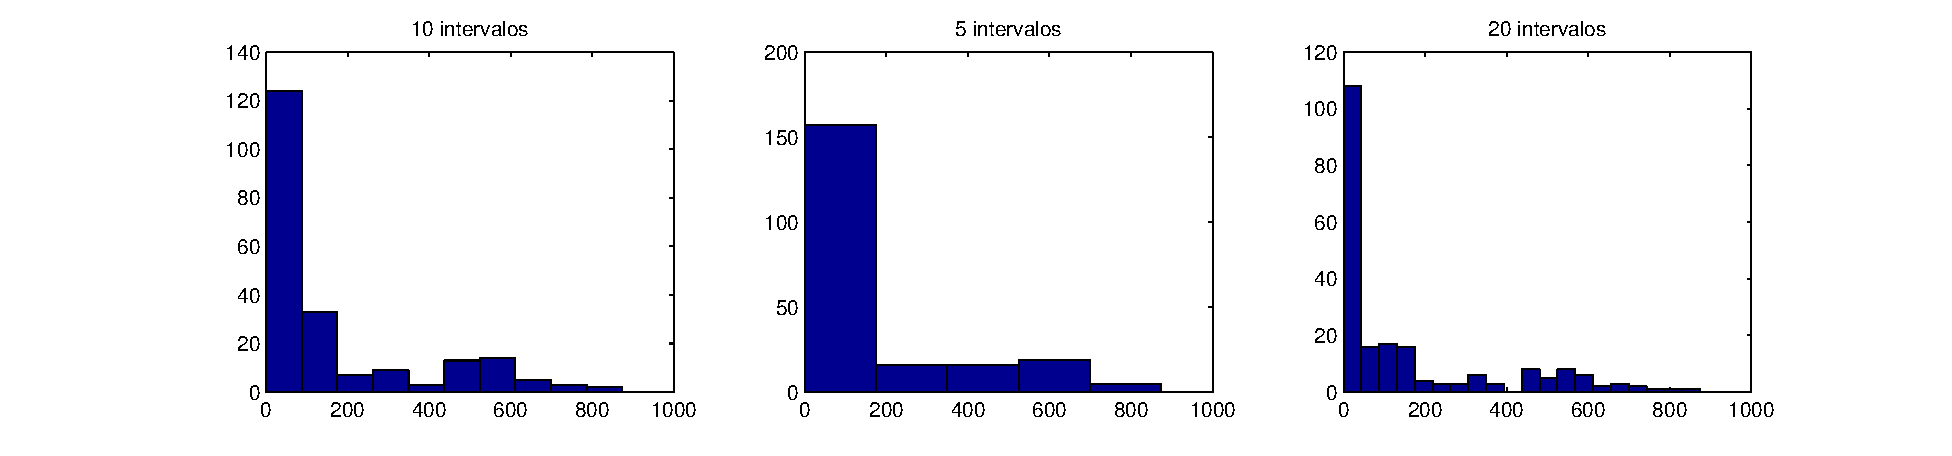
\includegraphics[width=15cm]{hist.eps}
\caption{histogramas del número de automóviles por cada 1000 habitantes para 213 países}
\label{fig:hist}
\end{figure}

La interpretación del los histogramas depende lógicamente del número de intervalos. En el caso de 10 intervalos, estos dividen los datos en grupos de aproximadamente 100 coches. Si observamos el histograma resultante, podemos concluir que hay unos 120 países en los que hay entre 0 y 100 automóviles por cada 1000 habitante, unos 30 países en los que hay entre 100 y 200 automóviles por cada 1000 habitante, etc. Si miramos el siguiente histograma, en el que se han empleado tan solo 5 intervalos, los grupos son ahora de aproximadamente 200 coches. La primera barra de este segundo histograma establece que hay unos 150 países en los que hay entre 0 y 200 coches por cada 1000 habitantes. Resultado que corresponde a la suma de los de dos primeros intervalos del histograma anterior. Para el tercer histograma los intervalos son ahora de 50 automóviles, lo que permite observar más en detalle que en los histogramas anteriores la distribución de vehículos: 110 países tienen menos de 50 automóviles por cada 1000 habitantes.

\paragraph{plotyy.} Este comando permite representar dos gráficas en la misma figura de modo que comparten el mismo eje x y cada una tiene su propio eje y. La figura \ref{fig:plotyy} muestra el resultado del siguiente ejemplo,

\begin{verbatim}
>> x1=linspace(0,10,100);
>> x2=linspace(0,12,50);
>> y1=x1.^2;
>> y2=x2.^(2/3);
>> plotyy(x1,y1,x2,y2)
>> grid on
\end{verbatim}

\begin{figure}[h]
\centering
\includegraphics[width=10cm]{plotyy.eps}
\caption{Ejemplo de uso de la función \texttt{plotyy}}
\label{fig:plotyy}
\end{figure}

\paragraph{quiver.} Esta función de Matlab permite dibujar vectores en el plano. En realidad está pensada para dibujar campos vectoriales, con lo que hay que manejarla con cierto cuidado. En primera aproximación diremos que \texttt{quiver} necesita 5 variables de entrada: la coordenada $x$ del origen del vector, la coordenada $y$ del origen del vector, la componente $x$ del vector y la componente $y$ del vector, por último, un factor de escala al que daremos el valor $0$ para que dibuje los vectores a su tamaño real, sin modificar su escala. Por ejemplo si queremos dibujar el vector $\vec{v}=(1,2)$ situado en el origen de coordenadas,
\begin{verbatim}
quiver(0,0,1,2,0)
\end{verbatim}

Si queremos representar el mismo vector pero situado en el punto $(3,-1)$,
\begin{verbatim}
>>quiver(3,-1,1,2,0)
\end{verbatim}

Podemos dibujar un conjunto de vectores con quiver, para ello empleamos como variables de entradas vectores, en lugar de escalares; un vector que contenga las posiciones $x$ del los orígenes, un segundo vector que contenga la posiciones $y$ de los orígenes, un tercer vector que contenga las componentes $x$ de los vectores y un cuarto que contenga las componentes $y$, por último añadiríamos el parámetro de escala $0$, que sigue siendo un escalar.

Por tanto, si queremos dibujar a la vez los dos vectores de los ejemplos anteriores,

\begin{verbatim}
>>quiver([0 3],[0 -1],[1 1],[2 2],0)
\end{verbatim}

La figura \ref{fig:quiver} muestra los resultados del ejemplo que acabamos de ver,

\begin{figure}[h]
\centering
\includegraphics[width=10cm]{quiver.eps}
\caption{Ejemplo de uso de la función \texttt{quiver}}
\label{fig:quiver}
\end{figure}

\paragraph{errorbar.} Permite añadir barras de  error a un gráfico de puntos experimentales. Supongamos que tenemos la siguiente tabla (\ref{vel}) de resultados de la medida de la velocidad de un móvil frente al tiempo,


\begin{table}[h]
\caption{Resultados experimentales de la medida de la velocidad de un móvil}
\centering
\begin{tabular}{ccc}
\hline
\hline
tiempo &velocidad& incertidumbre\\ 
$t$ (s)&$v$ (m/s)& $\pm \Delta v$ (m/s)\\
\hline
0&0&0\\
1&2.8&0.8\\
2&4.0&0.8\\
3&4.3&0.9\\
4&4.2&0.9\\
5&4.8&1.0\\
6&6.3&1.0\\
7&7.9&1.0\\
8&8.9&1.1\\
9&9.0&1.1\\
10&8.7&1.1\\
\hline
\hline
\end{tabular}
\label{vel}
\end{table} 

La primera columna representa el instante de tiempo en que se tomó la medida, la segunda columna representa el valor medido de la velocidad y la tercera columna la incertidumbre de cada medida de velocidad.

podemos emplear el comando \texttt(errorbar) para representar la velocidad frente al tiempo, añadiendo una barra de error en cada medida que represente la incertidumbre,

\begin{verbatim}
>> vel=[0 2.8 4.0 4.3 4.2 4.8 6.3 7.9 8.9 9.0 8.7]
vel =

  Columns 1 through 7

         0    2.8000    4.0000    4.3000    4.2000    4.8000    6.3000

  Columns 8 through 11

    7.9000    8.9000    9.0000    8.7000

>> inc=[0 0.8 0.8 0.9 0.9 1.0 1.0 1.0 1.1 1.1 1.1]
inc =

  Columns 1 through 7

         0    0.8000    0.8000    0.9000    0.9000    1.0000    1.0000

  Columns 8 through 11

    1.0000    1.1000    1.1000    1.1000

>> t=0:10
t =

     0     1     2     3     4     5     6     7     8     9    10

>> errorbar(t,vel,inc)
>> xlabel('tiempo s')
>> ylabel('velocidad m/s')
\end{verbatim}

EL resultado se muestra en la figura \ref{fig:error}. Es interesante hacer notar que la longitud total de cada barra de error es el doble del valor de la incertidumbre correspondiente al punto. Por ejemplo para $t=1s, v+\Delta v=2.8\pm 0.8 m/s$ la longitud de la barra de error es $2\cdot \Delta v=1.6 m/s$). El comando \texttt{errobar}, puede también emplearse para representar incertidumbres asimétricas. Para ello  es preciso suministrar dos vectores uno \texttt{U} para dibujar la parte superior de la barra de error y otro \texttt{L} para dibujar la parte inferior; \texttt{errorbar(x,y,L,U)}. 

\begin{figure}[h]
\centering
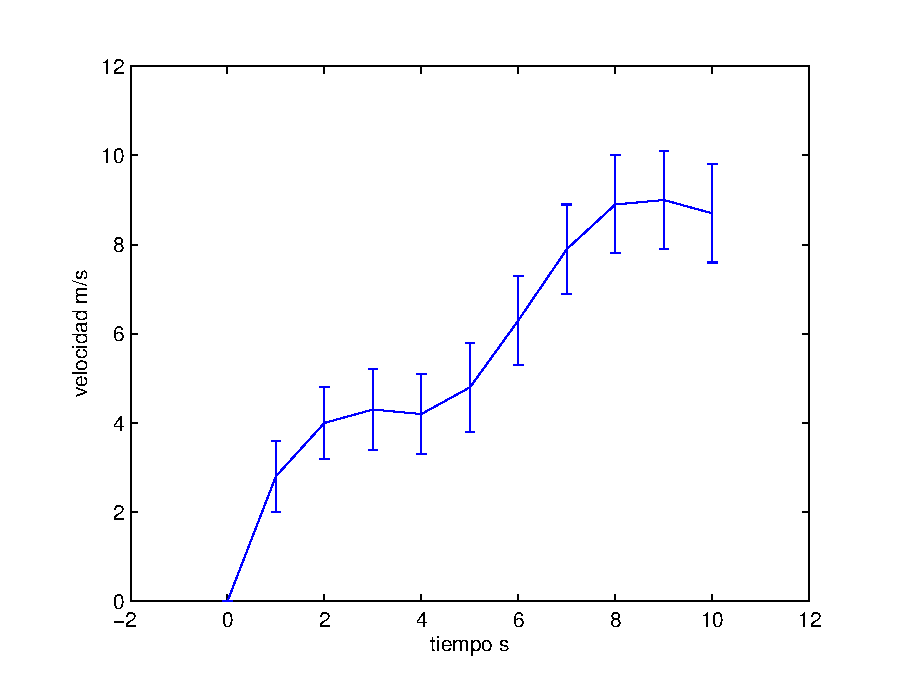
\includegraphics[width=11cm]{error.eps}
\caption{Datos de la tabla \ref{vel} representados empleando el comando \texttt{errorbar}}
\label{fig:error}
\end{figure}

\subsection{Gráficos en 3D.} \index{Gráficos! Comandos gráficos en 3D}En tres dimensiones es posible representar dos tipos de gráficos: puntos y curvas, análogos a los representados en dos dimensiones y además superficies en el espacio.

\paragraph{plot3.} Para dibujar líneas y puntos Matlab emplea los mismos comandos que hemos descrito para dos dimensiones, añadiendo al nombre de comando la terminación \texttt{3} para indicar que se trata de un gráfico en tres dimensiones. Así por ejemplo el comando \texttt{plot3} nos permite dibujar puntos y curvas en el espacio. El manejo es idéntico al de \texttt{plot}, simplemente que ahora es preciso añadir un vector que contenga los datos de la tercera coordenada, z. 

Por ejemplo, podemos representar la curva,
\begin{align*}
y&=\sin(2\pi x)\\
z&=\cos(2\pi x)
\end{align*}

Para ello, seleccionamos un intervalo de valores para $x \in (0,2)$, y calculamos los correspondientes valores de $y$ y $z$,

\begin{verbatim}
>> x=linspace(0,2,100);
>> y=sin(2*pi*x);
>> z=cos(2*pi*x);
\end{verbatim}

Podemos ahora representar la gráfica de nuestra función empleando el comando \texttt{plot3},
\begin{verbatim}
>> plot3(x,y,z)
>> grid on
>> xlabel('x')
>> ylabel('y')
>> zlabel('z')
\end{verbatim}

Hemos añadido los comandos \texttt{grid on}  para obtener una trama en 3D que permita ver mejor el resultado. La figura \ref{fig:muelle1} muestra la figura de Matlab obtenida, donde se ha señalado además un botón que permite rotar la figura, cambiando la vista. Para ellos, una vez pulsado el botón, basta con arrastrar el ratón sobre la figura manteniedo pulsado el boton izquierdo.  La figura \ref{fig:muelle2}, muestra la misma gráfica en 3D, pero ahora vista de frente (como si nos situáramos en el eje x). La figura \ref{fig:muelle3}, nos muestra la grafica vista desde arriba (desde el eje z), por último, la figura \ref{fig:muelle4} muestra una vista lateral de la gráfica (tomada desde el eje y).

Es posible rotar la figura par a obtener una vista concreta mediante el comando \texttt{view(Az, El)}. Este comando admite dos parámetros; \texttt{Az}, representa el azimuth o ángulo de rotación horizontal, \texttt{El}, representa el ángulo de elevación. Ambos ángulos se introducen en grados. Así, por ejemplo las vistas representadas en las figuras anteriores, se pueden obtener como,
\begin{verbatim}
>> view(90,0)
>> view(0,90)
>> view(0,0)
\end{verbatim}

\begin{figure}[h]
\centering
\subfigure[ventana gráfica \label{fig:muelle1}]{\includegraphics[width=6cm]{muelle1.png}} \qquad 
\subfigure[vista frontal (eje x) \label{fig:muelle2}]{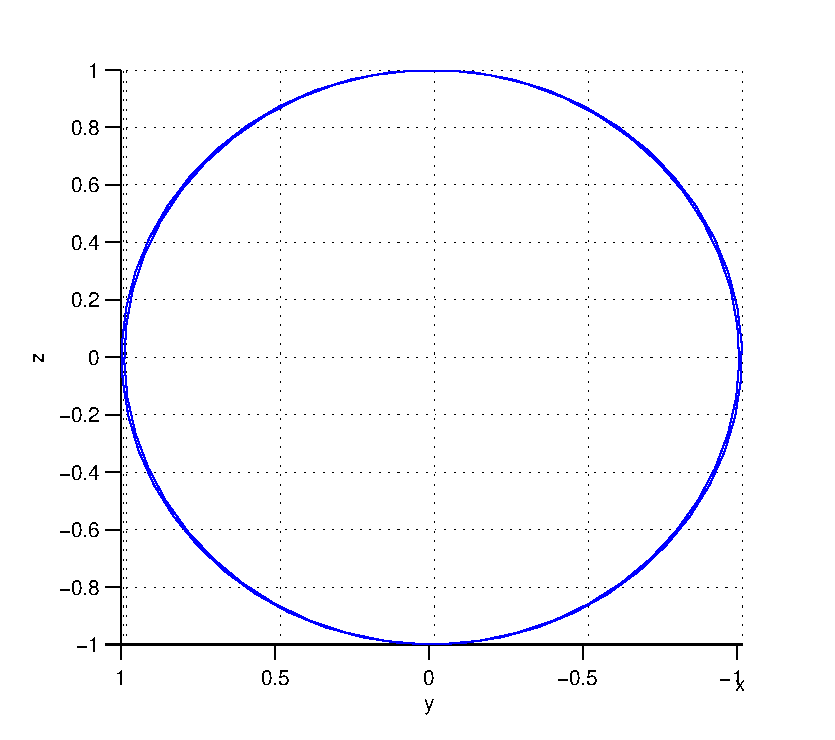
\includegraphics[width=6cm]{muelle2.eps}}\\
\subfigure[vista desde arriba (eje z) \label{fig:muelle3}]{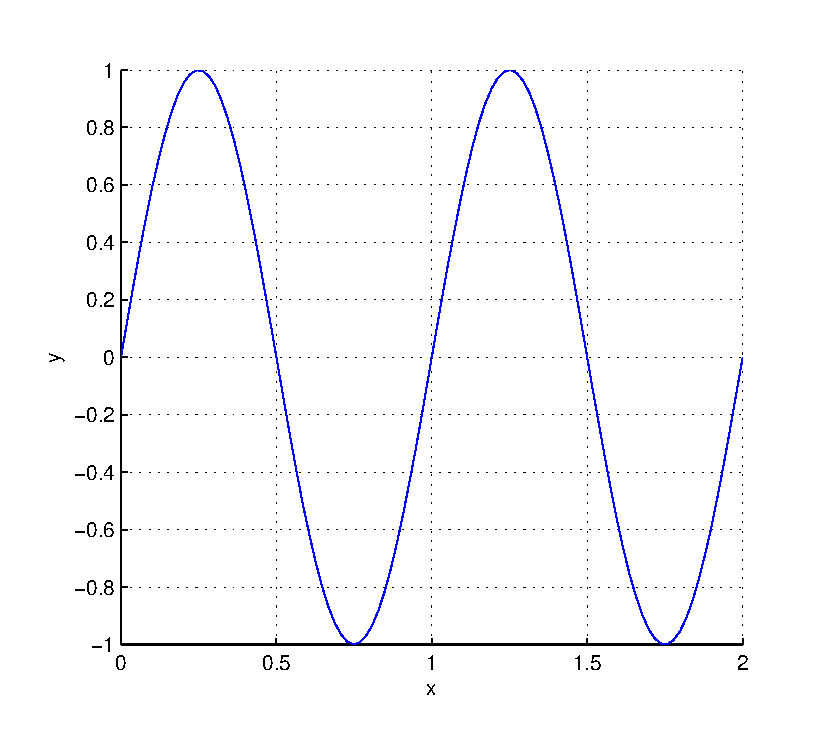
\includegraphics[width=6cm]{muelle3.eps}}\qquad
\subfigure[vista lateral (eje y)l \label{fig:muelle4}]{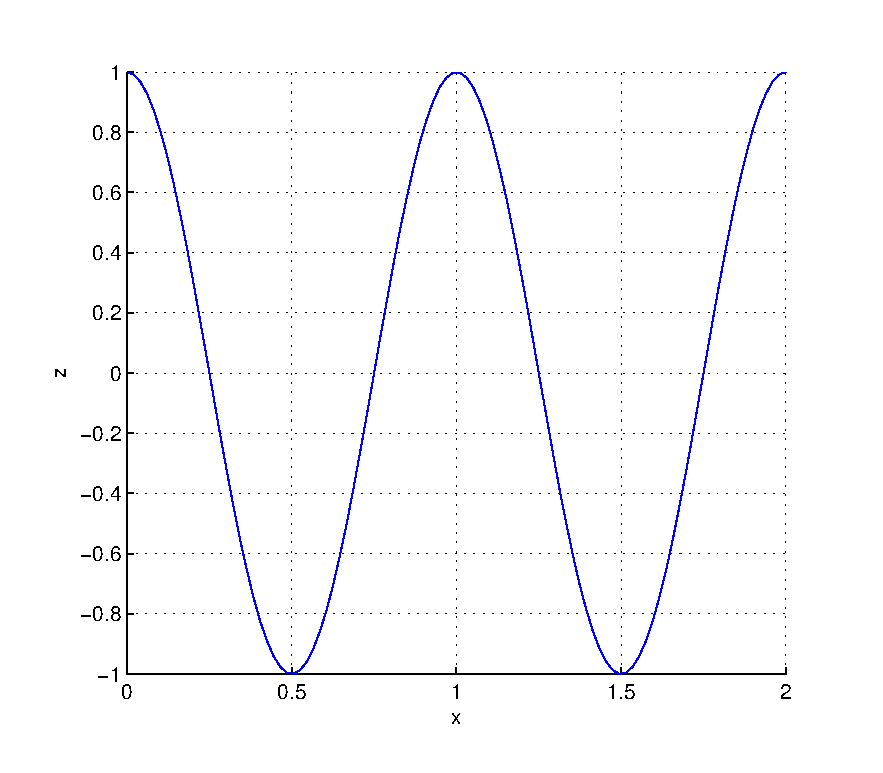
\includegraphics[width=6cm]{muelle4.eps}}\\
\caption{Gráfico en 3D y rotaciones. }
\end{figure}

\paragraph{bar3, stem3, hist3, quiver3.} Existen versiones 3D de los comandos \texttt{bar}, \texttt{stem}, \texttt{hist} y \texttt{quiver}. Su funcionamiento es similar ---aunque no siempre igual--- al de la versión 2D que vimos en la sección anterior. En algunos casos necesitan tres variables de entrada, correspondientes a las componentes (x,y,z) de los datos que se quiere representar, y en otros necesitan que los datos de entrada se le suministren en forma de matriz. Para conocer en detalle su funcinamiento, lo ideal es acudir a la ayuda de Matlab.


\paragraph{Superficies.}Para trazar superficies en el espacio, Matlab necesita en primer lugar que se defina una retícula en el plano $(x,y)$ que sirve de base sobre la que calcular los puntos z sobre los que se alzará la superficie.

Para definir dicha retícula Matlab emplea dos matrices. una de ellas $X_m$ contiene las coordenadas $x$ de los nodos de la retícula y la otra $Y_m$ las coordenadas $y$. Los elementos que ocupan la misma posición en ambas matrices, representan ---juntos--- un punto en el plano.
Matlab emplea dichas matrices como matrices de \emph{adyacencia}. Cada nodo, $(x_m(i,j),y_m(i,j)$, aparecerá en la gráfica conectado por una arista a cada uno de sus cuatros puntos vecinos, $(x_m(i-1,j),y_m(i-1,j)$, $(x_m(i,j-1),y_m(i,j-1)$, $(x_m(i+1,j),y_m(i+1,j)$, $(x_m(i,j+1),y_m(i,j+1)$.
Supongamos que empleamos las siguientes matrices, $X_m$ y $Y_m$ para definir una retícula sobre la que dibujar una superficie,

\begin{align*}
X_m=\begin{pmatrix}
0&1&2&3\\ 
0&1&2&3\\
0&1&2&3\\
0&1&2&3
\end{pmatrix},& Y_m\begin{pmatrix}
0&0&0&0\\
1&1&1&1\\
2&2&2&2\\
3&3&3&3
\end{pmatrix}\xrightarrow[nodos]{posiciones}\begin{matrix}
(0,0)&-&(1,0)&-&(2,0)&-&(3,0)\\
\vert&&\vert&&\vert&&\vert\\ 
(0,1)&-&(1,1)&-&(2,1)&-&(3,1)\\
\vert&&\vert&&\vert&&\vert\\
(0,2)&-&(1,2)&-&(2,2)&-&(3,2)\\
\vert&&\vert&&\vert&&\vert\\
(0,3)&-&(1,3)&-&(2,3)&-&(3,3)
\end{matrix}
\end{align*}

La retícula definida por Matlab, a partir de dichas matrices tendría el aspecto que se muestra en la figura \ref{fig:mesh}. 

\begin{figure}[h]
\centering
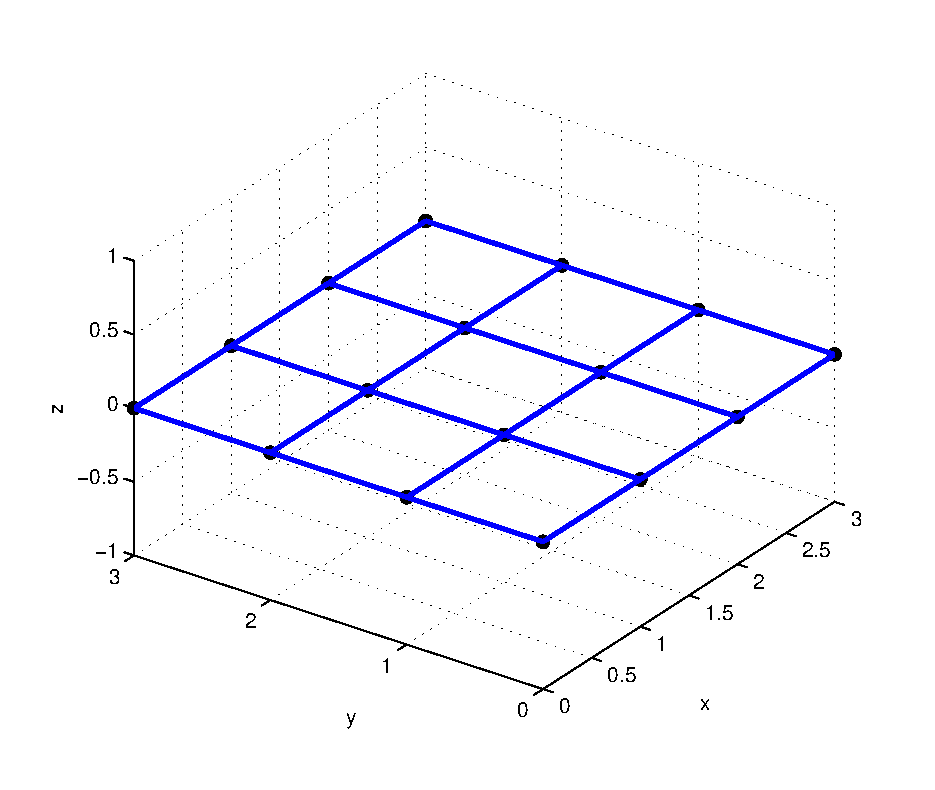
\includegraphics[width=11cm]{mesh.eps}
\caption{Retícula para representar superficies. Los puntos negros son los nodos definidos por las matrices $X_m$ e $Y_m$.}
\label{fig:mesh}
\end{figure}

Si nos fijamos en los ejes de la figura es fácil obtener las coordenadas de los nodos y comprobar como, están unidos entre sí por aristas los que ocupan posiciones adyacentes en las matrices $X_m$ e $Y_m$.

Para construir una superficie sobre la retícula, lo único que hace falta es definir una altura (z), para cada punto de la retícula. Para ello, Matlab emplea una matriz, del mismo tamaño que $X_m$ y $Y_m$. Así por ejemplo, si definimos,

\begin{equation*}
Z_m=\begin{pmatrix}
0&0&0&\\ 
0&1&2&0\\
0&3&4&0\\
0&0&0&0
\end{pmatrix}
\end{equation*}

Cada elemento de la matriz $Z_m$ representa la altura del nodo correspondiente a las posiciones marcadas por las matrices $X_m$ e $Y_m$, tal y como se muestra en la figure \ref{fig:mesh1}.

\begin{figure}[h]
\centering
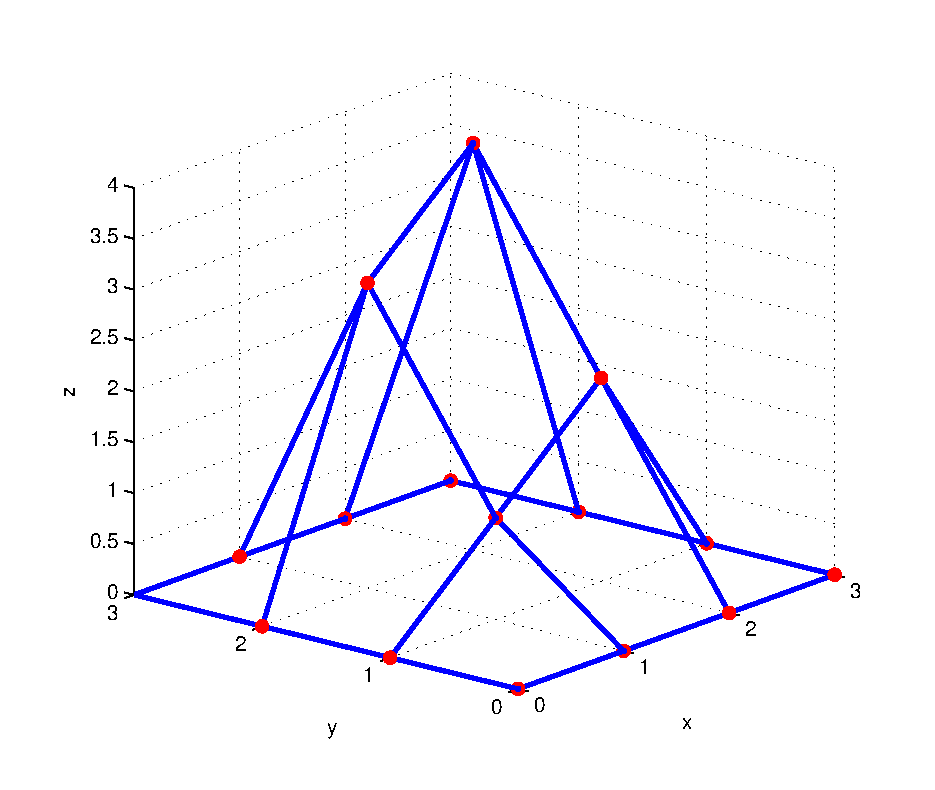
\includegraphics[width=11cm]{mesh1.eps}
\caption{Superficie elemental obtenida elevando los cuatros puntos centrales de la figura \ref{fig:mesh}.}
\label{fig:mesh1}
\end{figure}

La estructura de las matrices $X_m$ e $Y_m$ de los ejemplo anteriores, es la típica de las matrices de adyacencia de una retícula cuadrada; la matriz  $X_m$ tiene la filas repetidas y la matriz $Y_m$ tiene repetidas la columnas. En el ejemplo las matrices son cuadradas y definen una retícula de $4\times 4$ nodos. En general, podemos definir una retícula rectangular de $m\times n$ nodos. En este caso las matrices empleadas para definir la retícula tendrían dimensión $m\times n$.

Para dibujar en Matlab superficies podemos en primer lugar definir la retícula a partir de dos vectores de coordenadas empleando el comando \texttt{meshgrid}. En el ejemplo que acabamos de ver, hemos empleado una retícula que cubre el intervalo, $x\in[0,3]$ e $y\in[0,3]$. para definirlo creamos los vectores,

\begin{verbatim}
>> x=0:3
x =

     0     1     2     3

>> y=0:3
y =

     0     1     2     3
\end{verbatim}

A continuación empleamos el comando \texttt{meshgrid} para construir las dos matrices de adyacencia. Matlab se encargará de repetir las filas y columnas necesarias,

\begin{verbatim}
>> [Xm,Ym]=meshgrid(x,y)
Xm =

     0     1     2     3
     0     1     2     3
     0     1     2     3
     0     1     2     3


Ym =

     0     0     0     0
     1     1     1     1
     2     2     2     2
     3     3     3     3

\end{verbatim}

Una vez construidas las matrices de adyacencia, solo necesitamos una matriz de valores para $Z_m$. Si definimos por ejemplo,
\begin{verbatim}
>> Zm=zeros(size(Xm))

Zm =

     0     0     0     0
     0     0     0     0
     0     0     0     0
     0     0     0     0
\end{verbatim}

Podríamos representar la retícula plana de la figura \ref{fig:mesh}, empleando por ejemplo el comando \texttt{mesh(Xm, Ym, Zm)}.

\paragraph{mesh y surf.} Una vez que hemos visto como construir una retícula rectangular sobre la que construir una superficie, veamos como dibujarla con un ejemplo. Supongamos que queremos dibujar la superficie,
\begin{equation*}
z=x^3+y^2
\end{equation*}

En la región del plano, $x\in[-1.5,1.5]$, $y\in[-2,2]$. 

Igual que en el ejemplo inicial, lo primero que debemos hacer es construirnos una matrices de adyacencia que definan una retícula en la región de interés,
\begin{verbatim}
>> x=linspace(-1.5,1.5,25);
>> y=linspace(-2,2,50);
>> [Xm,Ym]=meshgrid(x,y);
\end{verbatim}

Es interesante notar que la región de interés no es cuadrada y que las matrices de adyacencia tampoco los son ($50\times 25$). Además los puntos no están espaciados igual en los dos ejes.

A continuación obtenemos la matriz de coordenadas z, aplicando la función a los puntos de la retícula,

\begin{verbatim}
>> Zm=Xm.^3+Ym.^2;
\end{verbatim}

\begin{figure}[h]
\centering
\subfigure[Función $z=x^3+y^2$ representada con \texttt{mesh}\label{fig:msh}]{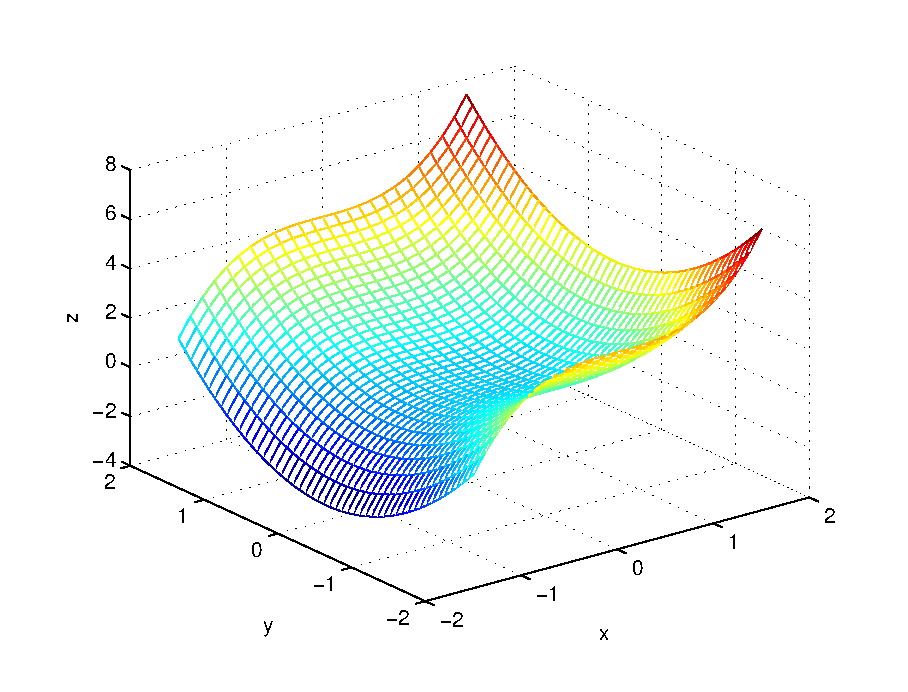
\includegraphics[width=8cm]{pa23.eps}} %\qquad 
\subfigure[Función $z=x^3+y^2$ representada con \texttt{surf} \label{fig:sur}]{\includegraphics[width=8cm]{surf.eps}}\\
\caption{Comparación entre \texttt{mesh} y \texttt{surf}}
\end{figure}

Para representar la superficie podemos emplear el comando \texttt{mesh}. 
\begin{verbatim}
>> mesh(Xm,Ym,Zm)
\end{verbatim}

Este comando admite como variables de entrada las dos matrices de adyacencia empleadas para definir la retícula y la matriz $Z_m$ que contiene los valores calculados para la  variable z, en todos los puntos de la retícula. \texttt{mesh} traza la superficie en forma reticular, es decir, nos dibuja una malla en el espacio. El color de la malla depende del valor que toma la coordenada z. Podemos también representar la superficie haciendo uso del comando \texttt{surf}, empleando las mismas variables de entrada que en el caso de \texttt{mesh}. 
\begin{verbatim}
>> surf(Xm,Ym,Zm)
\end{verbatim}

La diferencia está en que ahora la superficie muestra las caras definidas por la malla de colores, según el valor que toma la variable $z$. la figura \ref{fig:msh} muestra el resultado de nuestro ejemplo empleando \texttt{mesh} y la figura \ref{fig:sur} muestra el resultado empleando \texttt{surf}.



Para figuras que presentan simetría radial, puede ser más conveniente, definir las retículas en coordenadas polares. así por ejemplo,

\begin{verbatim}
>> r=0:2/20:2;
>> theta=0:2*pi/36:2*pi;
>> [rm,them]=meshgrid(r,theta);
\end{verbatim}

Hemos cosntruido una retícula en las variables $r$ y $\theta$, si ahora definimos las matrices de adyacencia como las proyecciones sobre los ejes $x$ e $y$,

\begin{verbatim}
>> xm=rm.*cos(them);
>> ym=rm.*sin(them); 
\end{verbatim}

Obtenemos una retícula con simetría radial, centrada en el origen de coordenadas. Como la que se muestra en la figura, \ref{fig:retcir}.

\begin{figure}[h]
\centering
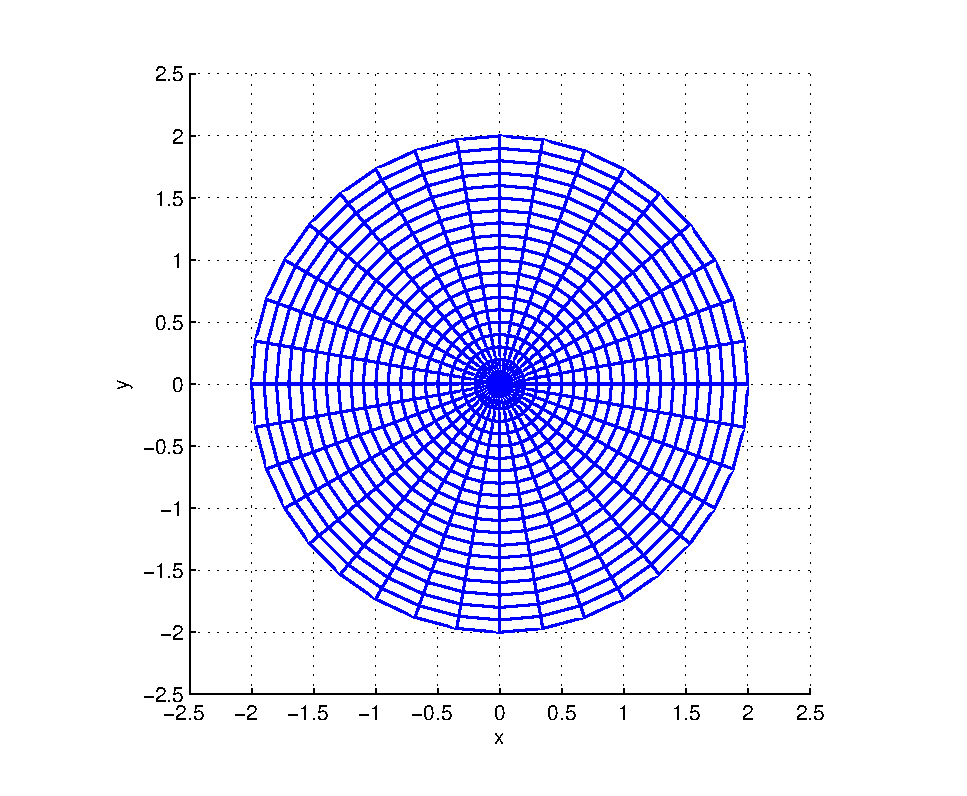
\includegraphics[width=12cm]{retcirc.eps}
\caption{retícula con simetría circular}
\label{fig:retcir}
\end{figure}

La retícula resulta muy adecuada para dibujar por ejemplo un cono (figura \ref{fig:cono}),

\begin{verbatim}
>> zm=2-sqrt(xm.^2+ym.^2);
>> mesh(xm,ym,zm)
\end{verbatim}

\begin{figure}[h]
\centering
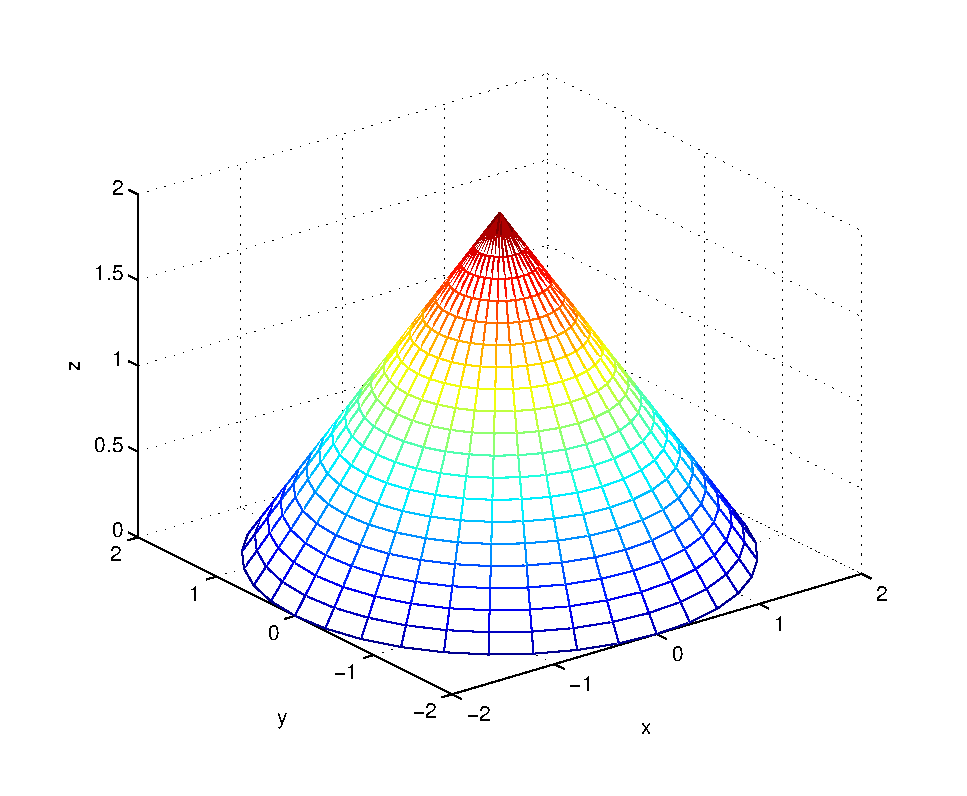
\includegraphics[width=12cm]{cono.eps}
\caption{Cono representado sobre una retícula circular}
\label{fig:cono}
\end{figure}

A continuación, se incluye el código de un script con varios ejemplos más de diseño de retículas circulares y gráficos de superficies en 3D. Los resultados se muestran en la figura \ref{fig:varios}

%\lstinputlisting{../codigo/matlab/introduccion/varios_g3d.m}

\begin{figure}[h]
\centering
\includegraphics[width=12cm]{varios.eps}
\caption{retícula con simetría circular}
\label{fig:varios}
\end{figure}

\paragraph{contour, contour3, meshc y surfc.} Este comandos permiten obtener y dibujar las curvas de nivel de una superficie. Su uso es idéntico al de los comandos anteriores. Es decir, también necesitan que se defina una retícula en el plano $(x,y)$, y se calculen los valores que tomará  la variable z sobre los puntos de la retícula.

\begin{figure}
\centering
\subfigure[contour  \label{fig:contour}]{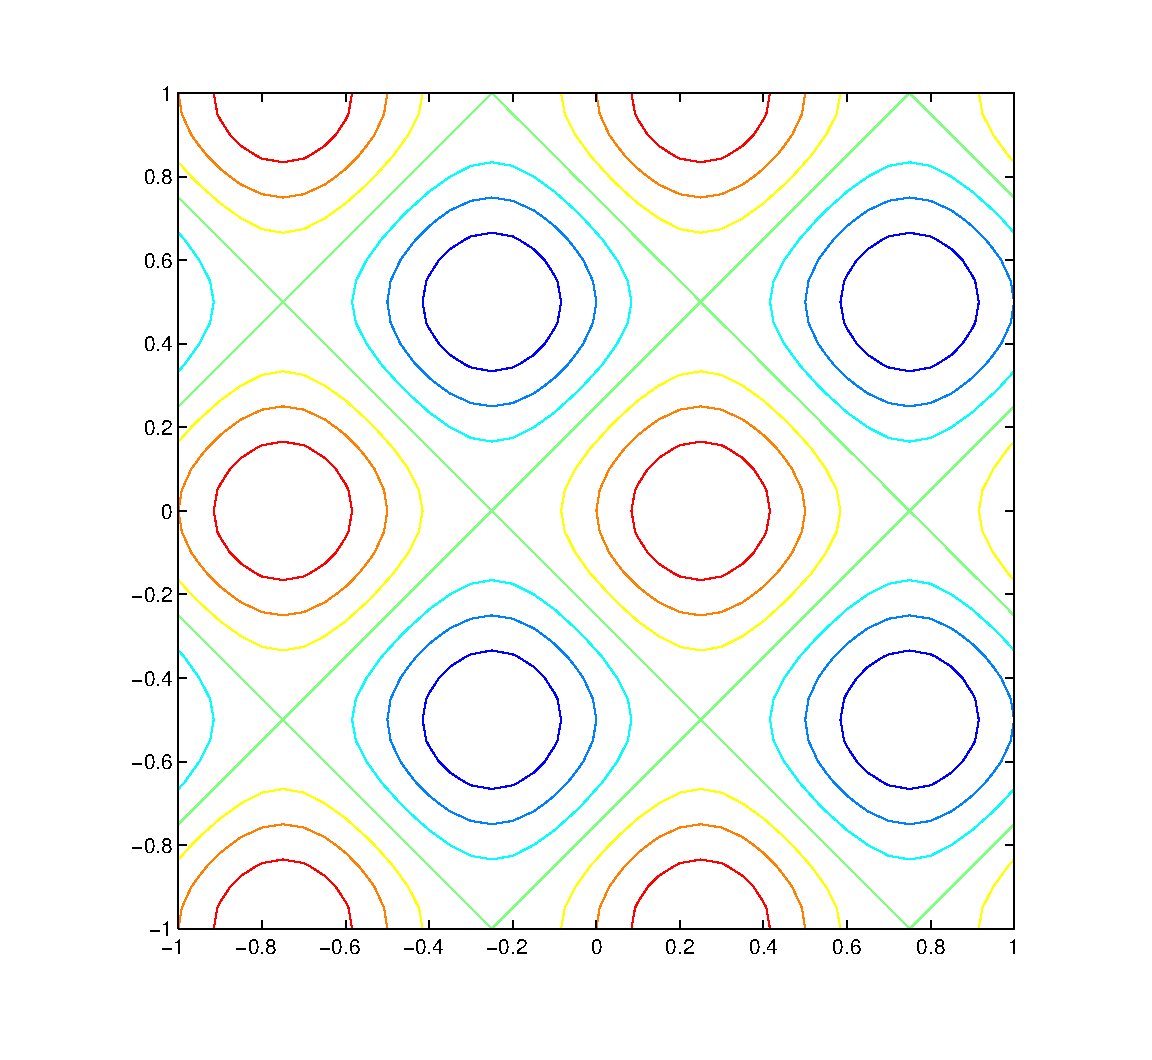
\includegraphics[width=6.5cm]{contour.eps}} \qquad 
\subfigure[contour3 \label{fig:contour3}]{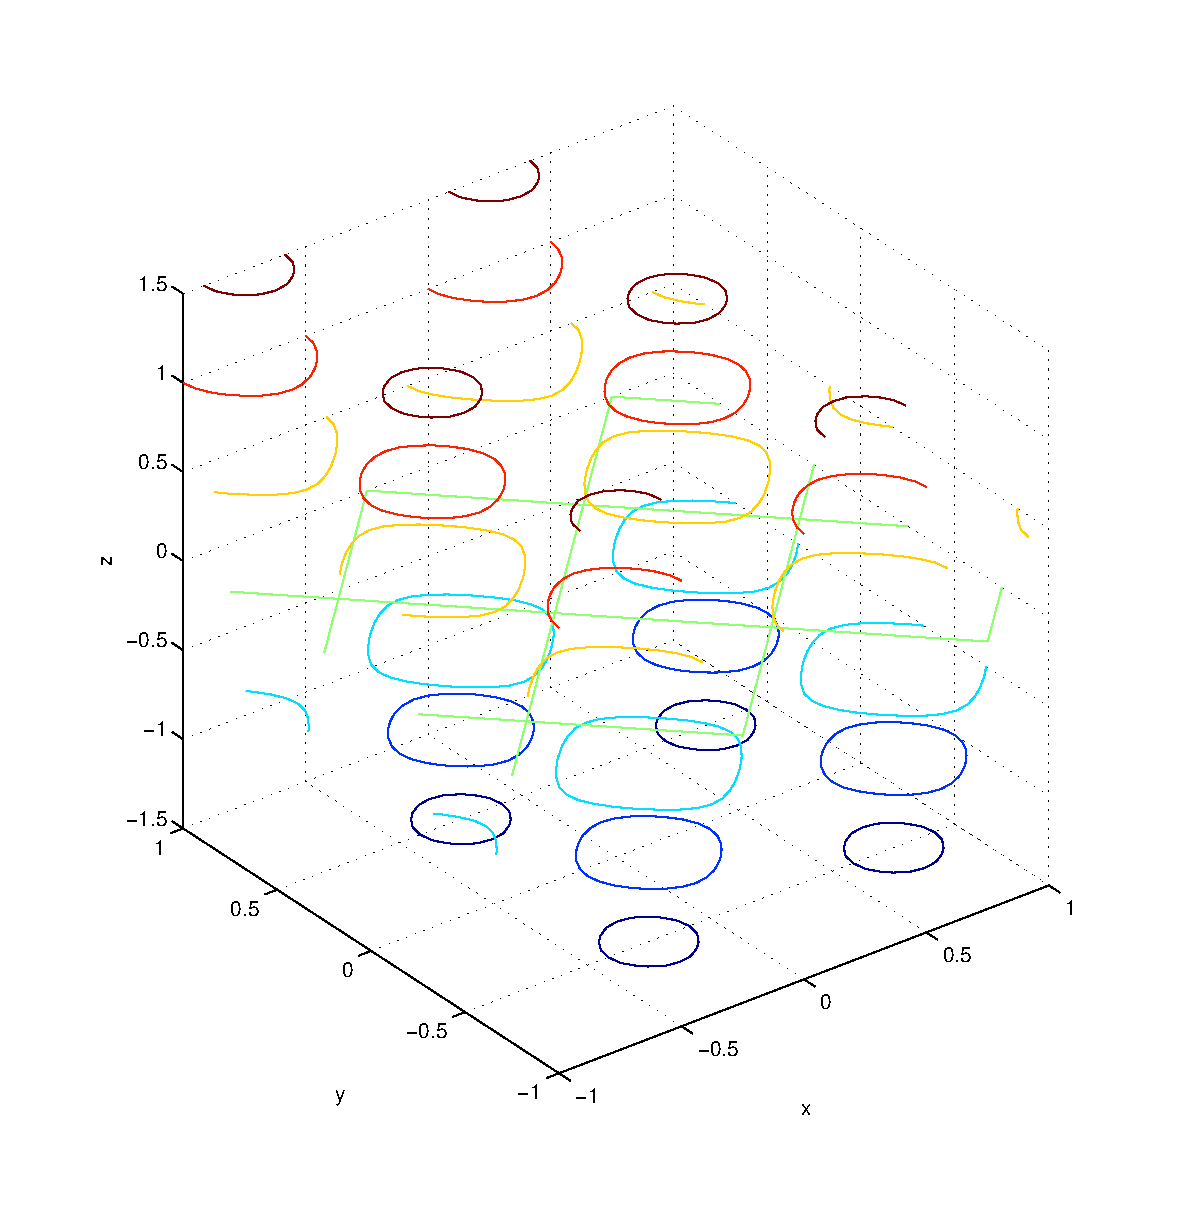
\includegraphics[width=6.5cm]{contour3.eps}}\\
\subfigure[meshc \label{fig:mesh3}]{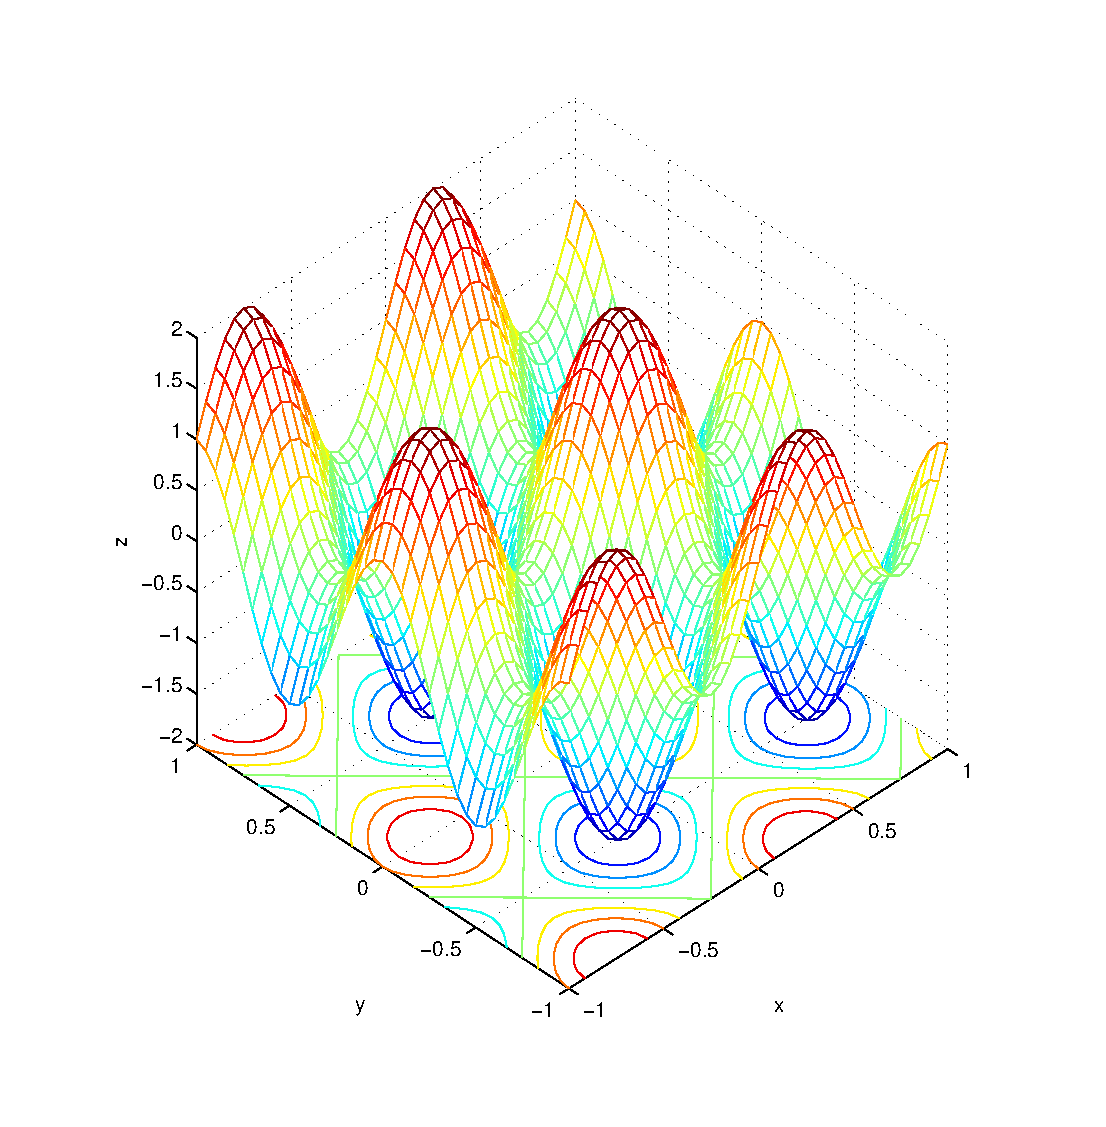
\includegraphics[width=6.5cm]{meshc.eps}}\qquad
\subfigure[surfc \label{fig:surf3}]{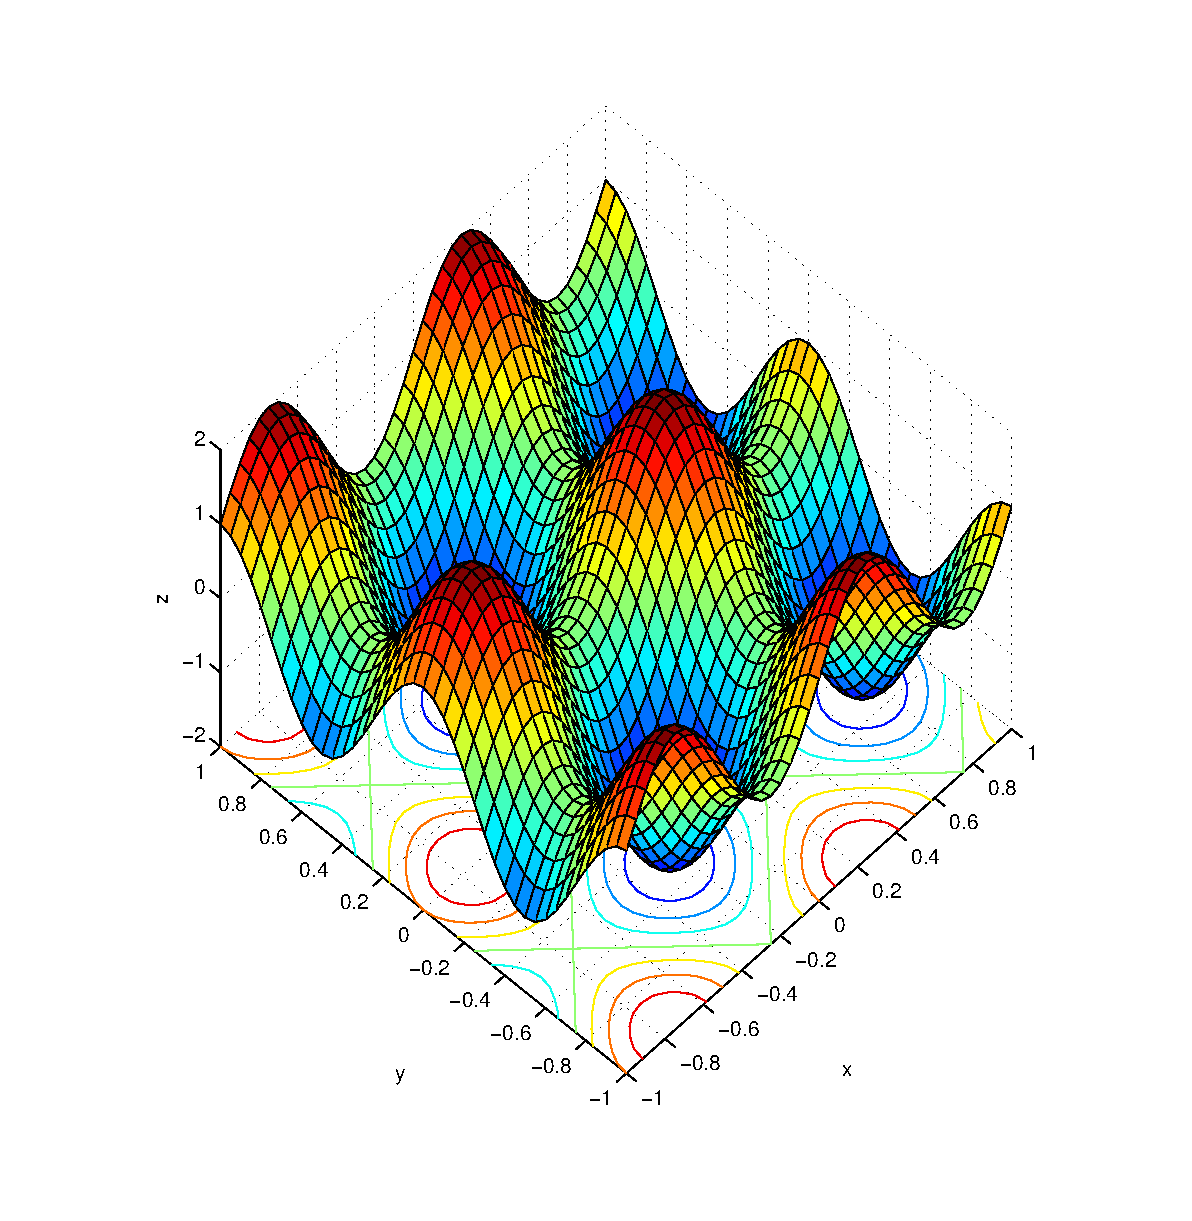
\includegraphics[width=6.5cm]{surfc.eps}}\\
\caption{Comparación entre los resultados de \texttt{contour}, \texttt{contour3}, \texttt{meshc} y \texttt{surfc}, para la obtención de las curvas de nivel de una superficie. }
\end{figure}

Veamos su funcionamiento con un último ejemplo. Obtenemos una retícula cuadrada, calculamos sobre ella los puntos de la superficie,

\begin{equation*}
z=\sin(2\pi x)+cos(2\pi y)
\end{equation*}

\begin{verbatim}
>> x=[-1:0.05:1];
>> y=x;
>> [xm,ym]=meshgrid(x,y);
>> zm=sin(2*pi*xm)+cos(2*pi*ym);
>> contour(xm,ym,zm)
>> contour3(xm,ym,zm)
>> meshc(xm,ym,zm)
>> surfc(xm,ym,zm)
\end{verbatim}



La figura \ref{fig:contour} muestra los resultados de aplicar el comando \texttt{contour}. La gráfica representa las curvas de nivel de la superficie dibujadas sobre el plano $(x,y)$. El comando \texttt{contour3} ( figura \ref{fig:contour3}) representa de nuevo las curvas de nivel, pero sitúa cada una a su correspondiente altura $z$.  Por último \texttt{meshc} y \texttt{surfc} representan la superficie y añaden en el plano $(x,y)$ la representación de las curvas de nivel correspondiente a la superficie.

Para terminar la sección dedicada a los gráficos, vamos a combinar el comando \texttt{mesh} con el comando \texttt{plot3} para dibujar una curva sobre una superficie. Tomaremos como ejemplo la superficie,
\begin{equation*}
z=\frac{sin\left((\pi x)^2+(\pi y^2)\right)}{(\pi x)^2+(\pi y^2)}
\end{equation*}

Sobre la que trazamos la curva,

\begin{equation*}
y=sin(\pi x),\\
\end{equation*}

\begin{figure}[h]
\centering
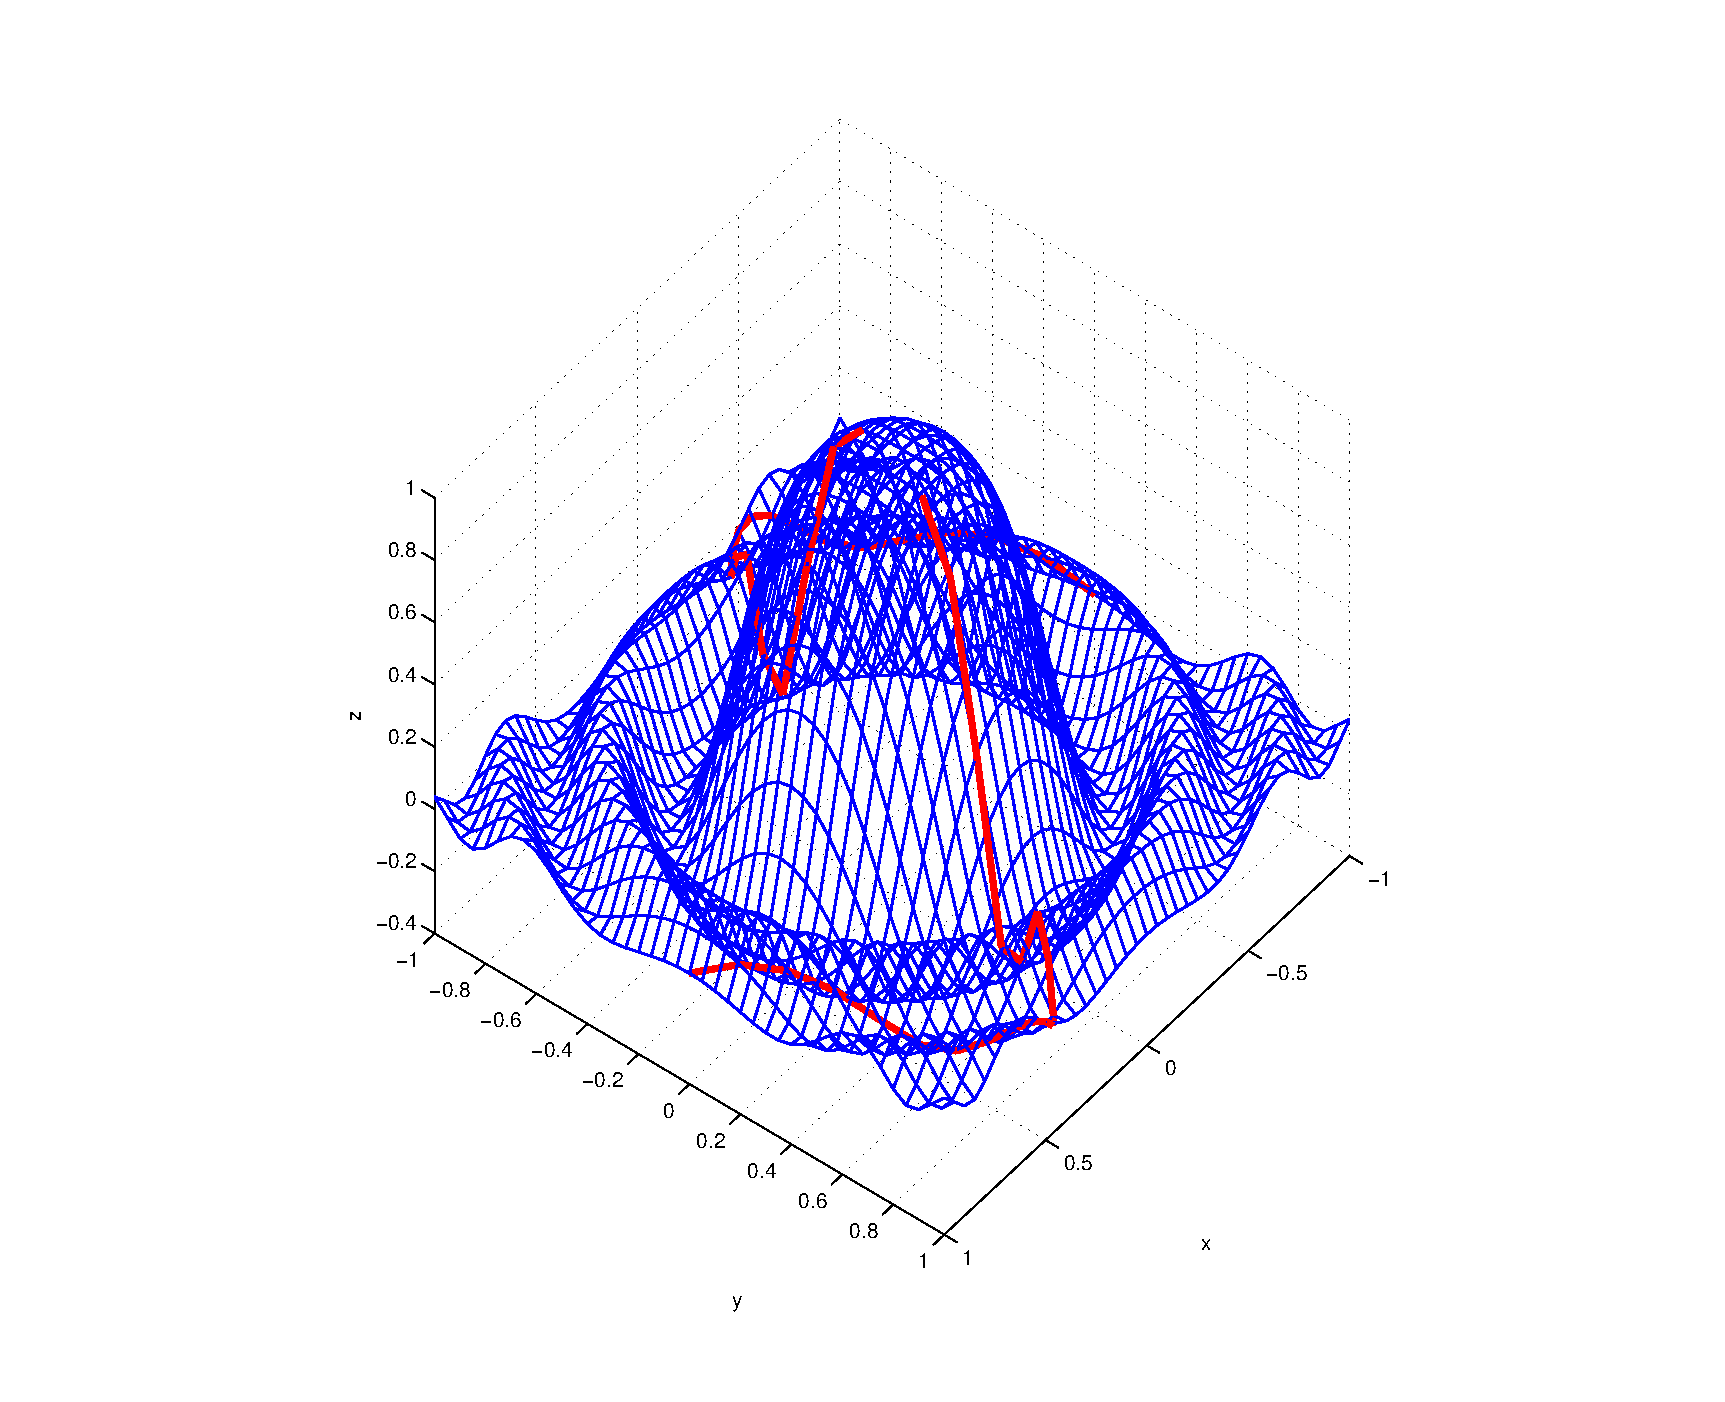
\includegraphics[width=11cm]{linsu.eps}
\caption{Curva trazada sobre una superficie}
\label{fig:cvsurf}
\end{figure}

Es decir, obtenemos el valor de los puntos $z$ de la superficie para los pares de puntos $[x, y = sin(\pi x)]$, que definen la curva trazada sobre la superficie $z$,

\begin{verbatim}
>> x=[-1:0.05:1];
>> y=x;
>> [xm,ym]=meshgrid(x,y);
>> zm=sin((pi*xm).^2+(pi*ym).^2)./((pi*xm).^2+(pi*ym).^2);
>> mesh(xm,ym,zm)
>> y=sin(pi*x);
>> z=sin((pi*x).^2+(pi*y).^2)./((pi*x).^2+(pi*y).^2);
>> hold on
>> plot3(x,y,z)
\end{verbatim}

Es importante insistir en que a lo largo de esta sección nos hemos limitado a introducir algunas de las posibilidades gráficas de Matlab. Para obtener una visión completa de las mismas es imprescindible leer con detenimiento la ayuda de Matlab.
